\documentclass[11pt]{article}
\usepackage[margin=1in]{geometry}
\usepackage{amsmath,amssymb,amsthm}
\usepackage{graphicx}
\usepackage{hyperref}

\newtheorem{theorem}{Theorem}
\newtheorem{lemma}{Lemma}
\newcommand{\R}{\mathbb R}
\newcommand{\Gr}{\operatorname{Gr}}
\newcommand{\cH}{\mathcal H}
\newcommand{\cM}{\mathcal M}
\newcommand{\cA}{\mathcal A}
\newcommand{\cP}{\mathcal P}

\title{Periodic-jet monodromy refutes the higher-order\\
M-bundle section conjecture}
\author{A counterexample to the conjecture after Theorem 3.5 of arXiv:2310.13115}
\date{11 August 2026}

\begin{document}
\maketitle

\noindent\textbf{Status.}
\texttt{candidate\_full\_counterexample\_likely\_valid\_needs\_human\_review}.

\begin{abstract}
O'Neill proves that a nontrivial, Glaeser-stable, proper, consistent
M-bundle has a manifold section whenever its associated Grassmannian bundle
has a continuous section and the jet order is \(m=1\), and conjectures the
same for \(m\ge2\). We disprove the conjecture for every \(m\ge4\). On a
circle in \(\R^3\), all allowed jets have the same horizontal tangent plane
and vanish through order \(m-2\). Their free \((m-1)\)-st radial coefficient
\(b\) is locally constrained at order \(m\) by \(b'=1\). Every allowed jet
has a local realization, so the M-bundle is Glaeser-stable; nevertheless, a
global manifold section would make \(b\) a periodic \(C^1\) function with
derivative one. The vanishing lower jets ensure that changes of graph
coordinates act affinely through order \(m\), which is the key point needed
for the construction to be an M-bundle.
\end{abstract}

\section{Source conjecture}

For a compact \(E\subset\R^n\), an M-bundle is a family

\[
 H(x)\subset O(n)\times\cP^m(\R^d,\R^{n-d})
\]

whose fixed-coordinate fibers \(H^Q(x)=\{P:(Q,P)\in H(x)\}\) are affine
spaces (empty fibers are allowed). It is \emph{proper} when every graph jet
passes through \(x\), and \emph{consistent} when a jet belongs to every
other graph coordinate system in which the same geometric jet can be
realized. Its associated Gr-bundle records the tangent \(d\)-planes.

A section of the M-bundle is a \(C^m\) manifold \(\cM\supset E\) whose local
graph jet at every \(x\in E\), in every compatible graph coordinate system,
lies in \(H(x)\). Theorem 3.5 of \cite{source} proves that a nontrivial,
Glaeser-stable, proper, consistent M-bundle has a section for \(m=1\),
provided its Gr-bundle has a continuous section. The sentence immediately
following the theorem conjectures this for \(m\ge2\); see
Figure~\ref{fig:source}.

\section{The affine jet family}

Fix an integer \(m\ge4\), set \(d=2,n=3\), and let

\[
 E=\{x_t=(\cos t,\sin t,0):t\in\R/(2\pi\mathbb Z)\}.
\]

Let \(T=\R^2\times\{0\}\). Near the planar unit circle, use tubular
coordinates

\[
 \vartheta=\arg(x+iy),\qquad
 \sigma=\sqrt{x^2+y^2}-1.
\]

Near \(x_t\), choose the lift of \(\vartheta\) for which
\(\vartheta-t=0\) at \(x_t\). For \(b,c\in\R\), define the local height

\begin{equation}\label{eq:local-model}
 \Phi_{t,b,c}(\vartheta,\sigma)
 =\frac{(b+\vartheta-t)\sigma^{m-1}}{(m-1)!}
  +\frac{c\sigma^m}{m!}.
\end{equation}

Let

\[
 \cA_t=\{J^m_{x_t}\Phi_{t,b,c}:b,c\in\R\}.
\]

This is an affine two-parameter family of scalar \(m\)-jets. Every member
has value zero, horizontal gradient zero, and all derivatives of orders
\(2,\ldots,m-2\) equal to zero. In particular, every graph has tangent plane
\(T\).

Use \(I\) for the standard graph coordinates over \(T\), and put
\(H^I(x_t)=\cA_t\). For \(Q\in O(3)\), let \(\pi_Q\) denote projection onto
the first two \(Q\)-coordinates. If \(\pi_Q|_T\) is invertible, define
\(H^Q(x_t)\) to be all \(Q\)-coordinate realizations of the geometric jets
in \(\cA_t\). If \(\pi_Q|_T\) is singular, set \(H^Q(x_t)=\varnothing\).
Finally, let

\[
 H(x_t)=\bigcup_{Q\in O(3)}\{Q\}\times H^Q(x_t).
\]

The following calculation verifies the non-obvious M-bundle axiom.

\begin{lemma}[Affine coordinate realization]\label{lem:affine}
Let \(m\ge4\). Among scalar graph jets with a fixed tangent plane and with
all nonlinear terms of degrees below \(m-1\) equal to zero, realization in
any other graph coordinate system is affine-linear through degree \(m\).
Consequently every \(H^Q(x_t)\) above is an affine space.
\end{lemma}

\begin{proof}
Center both coordinate systems at the point in question and start in
coordinates adapted to \(T\). Write the height as

\[
 f(u)=f_{m-1}(u)+f_m(u)+o(|u|^m),\qquad u\in\R^2,
\]

where \(f_j\) is homogeneous of degree \(j\). In the new orthogonal
coordinates, split the rigid linear map into independent and dependent
blocks:

\[
 y=Au+a f(u),\qquad v=c^{\mathsf T}u+\gamma f(u),
\]

with \(A\in\R^{2\times2}\), \(a,c\in\R^2\), and \(\gamma\in\R\).
Compatibility with the tangent plane is exactly invertibility of \(A\).
Put \(B=A^{-1}\). Formal inversion through degree \(m\) gives

\begin{equation}\label{eq:inverse}
 u=By-Ba\bigl[f_{m-1}(By)+f_m(By)\bigr]+o(|y|^m).
\end{equation}

Indeed, substituting the correction of degree \(m-1\) back into
\(f_{m-1}\) first changes it in degree
\((m-2)+(m-1)=2m-3>m\); all other omitted interactions occur still later.
Using \eqref{eq:inverse}, the new graph height is

\begin{equation}\label{eq:transform}
 v=c^{\mathsf T}By+
   (\gamma-c^{\mathsf T}Ba)
   \bigl[f_{m-1}(By)+f_m(By)\bigr]+o(|y|^m).
\end{equation}

Thus the transformed \(m\)-jet depends linearly on the two varying
homogeneous pieces, in addition to its fixed linear part. The family
\(\cA_t\) is affine in those pieces, so its image is affine.
\end{proof}

\section{Proof intuition}

The circle hides a local-to-global obstruction that Glaeser refinement
cannot see. At each base point one may freely choose \(b\), then realize the
nearby fibers by increasing that coefficient at unit speed. This supplies
all finite-point Taylor compatibility tests in a neighborhood. Going once
around the circle, however, unit-speed increase cannot return to its initial
value.

Placing \(b\) in order \(m-1\), rather than in the tangent or curvature,
serves a second purpose. It makes the first possible nonlinear interaction
under a change of graph coordinates have degree \(2m-3\). For \(m\ge4\)
this lies beyond the retained \(m\)-jet, so fixed-coordinate fibers remain
affine.

\section{Counterexample theorem}

\begin{theorem}\label{thm:counterexample}
For every integer \(m\ge4\), the family
\(\cH=(H(x))_{x\in E}\) constructed above is a nontrivial,
Glaeser-stable, proper, consistent M-bundle. Its associated Gr-bundle has
the constant section \(x\mapsto T\), but \(\cH\) has no manifold section.
Hence the conjecture following Theorem 3.5 of \cite{source} is false.
\end{theorem}

\begin{proof}
Lemma~\ref{lem:affine} proves that every \(H^Q(x)\) is affine, so \(\cH\)
is an M-bundle. It is nontrivial because \(H^I(x_t)=\cA_t\ne\varnothing\).
Every jet is the jet of a graph through \(x_t\), so the bundle is proper.
All jets have tangent \(T\); hence the associated Grassmannian fiber is the
singleton \(\{T\}\), and \(x\mapsto T\) is a continuous section.

Consistency holds by construction. Namely, an element of \(H^Q(x_t)\) is
the \(Q\)-realization of a geometric jet from \(\cA_t\). If that graph jet
is compatible with another coordinate system \(R\), its tangent is \(T\),
so \(\pi_R|_T\) is invertible; its \(R\)-realization belongs to
\(H^R(x_t)\) by definition.

We next prove Glaeser stability. Fix \(t_0,b_0,c_0\). On a sufficiently
short arc around \(t_0\), use the single smooth height

\[
 \Phi(\vartheta,\sigma)=
 \frac{(b_0+\vartheta-t_0)\sigma^{m-1}}{(m-1)!}
 +\frac{c_0\sigma^m}{m!}.
\]

At \(x_s\) in this arc, rewrite

\[
 b_0+\vartheta-t_0=(b_0+s-t_0)+(\vartheta-s).
\]

Therefore \(J^m_{x_s}\Phi\in\cA_s\), and the jet at \(x_{t_0}\) is the
arbitrarily prescribed member corresponding to \(b_0,c_0\). In every
compatible \(Q\)-coordinate system, the same local surface is the graph of
a \(C^m\) function and its jets lie in \(H^Q(x_s)\). Taylor's theorem gives
exactly the finite-point estimates in the definition of Glaeser refinement.
Thus every element of every nonempty fixed-\(Q\) fiber survives refinement.
Empty fixed-\(Q\) fibers are empty for all \(x_t\) and remain so. Hence
\(\cH\) is Glaeser-stable.

Suppose, for contradiction, that \(\cM\supset E\) were a manifold section.
At every \(x_t\), its tangent plane must be \(T\), so the sheet through \(E\)
is locally a height graph over the horizontal plane. These local height
germs agree on overlaps. Define

\[
 b(t)=\partial_\sigma^{m-1}F(\vartheta,0)\big|_{\vartheta=t},
\]

using any such local height \(F\). This is a well-defined, \(2\pi\)-periodic
\(C^1\) function because \(\cM\) is \(C^m\). Since the standard-coordinate
jet belongs to \(\cA_t\), equation \eqref{eq:local-model} gives

\[
 b'(t)=
 \partial_\vartheta\partial_\sigma^{m-1}F(t,0)=1.
\]

Integrating once around the circle yields

\[
 0=b(2\pi)-b(0)=\int_0^{2\pi}b'(t)\,dt=2\pi,
\]

a contradiction. Thus \(\cH\) has no section.
\end{proof}

\section{Scope and verification}

The construction refutes the universal statement ``for \(m\ge2\)'' by
giving counterexamples for every \(m\ge4\). It does not decide the isolated
orders \(m=2\) or \(m=3\). At \(m=3\), the degree identity becomes
\(2m-3=m\), so a quadratic coordinate-change interaction enters the retained
jet; the affine-fiber argument above no longer applies.

The accompanying exact symbolic checker verifies the formal inverse and
coordinate-change formula on deterministic rational polynomial instances,
the threshold inequality \(2m-3>m\), and the mixed derivative in
\eqref{eq:local-model}. These checks guard against degree and sign errors but
do not replace the proof. Four lightweight run indexes and bounded arXiv
searches found no duplicate or later resolution through 11 August 2026.
Human review should focus on Lemma~\ref{lem:affine}, the fixed-\(Q\) Glaeser
stability argument, and the passage from local height germs to the periodic
coefficient \(b\).

\begin{thebibliography}{9}
\raggedright
\bibitem{source}
K. O'Neill,
\emph{A Whitney Extension Problem for Manifolds},
arXiv:2310.13115 (2023), Theorem 3.5 and the following conjecture.
\end{thebibliography}

\begin{figure}[ht]
\centering
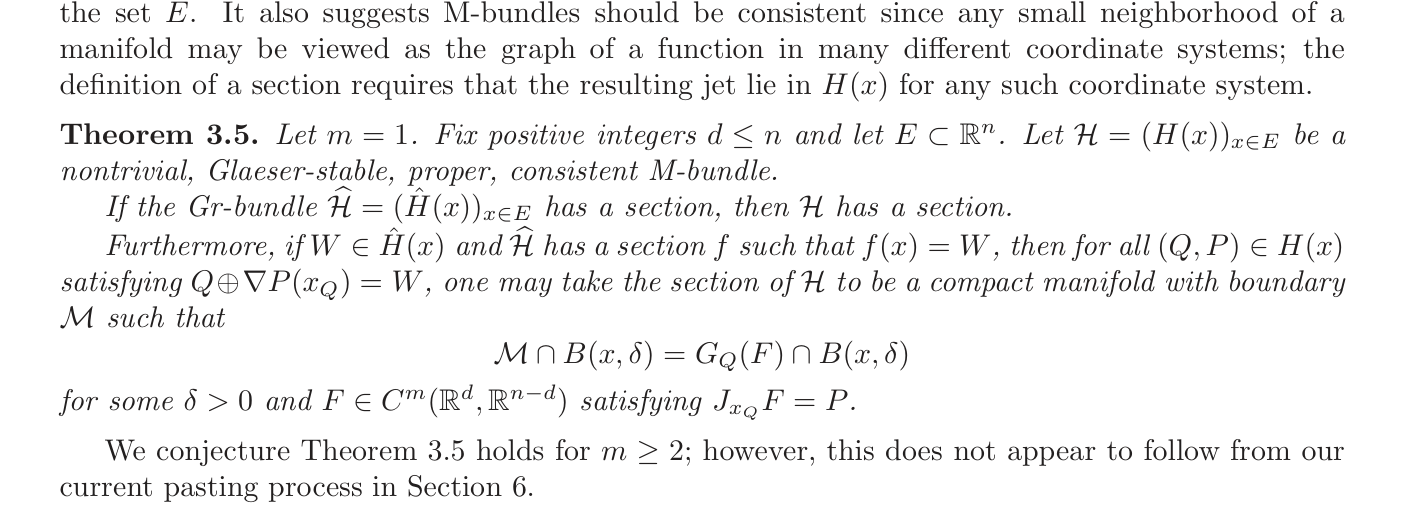
\includegraphics[width=0.94\textwidth]{figures/source_conjecture.png}
\caption{Source PDF page 15: Theorem 3.5 and the conjectured extension to
\(m\ge2\).}
\label{fig:source}
\end{figure}

\end{document}
